\newcommand{\packedTagResultsAucTable}{
    \begin{table}[H]
        \centering
        \begin{tabular}{|p{2,8cm}||P{2,2cm} P{2,2cm} P{2,2cm} P{2,2cm}|}
            \hline
            Packed Tag & ALOHA\newline (M/B only) & ALOHA & Joint\newline Embedding & Proposed\newline Model \\
            \hline
            AUC-ROC & - & 0.978$\pm$0.003 & 0.980$\pm$0.001 & \textBF{0.982$\pm$0.001} \\
            \hline
        \end{tabular}
        \caption[Packed Tag prediction task AUC-ROC results]{AUC-ROC (Area Under Curve) of the different models for the \textbf{Packed Tag} prediction task. Results were aggregated over \textBF{3} training runs with different weight initializations and minibatch orderings. Best results are shown in \textbf{bold}.} \label{tab:packedTag_auc}
    \end{table}
}

\newcommand{\packedTagResultsAtFprTable}{
    \begin{center}
        \begin{longtable}[c]{|P{3,2cm}||P{1,8cm} P{1,8cm} P{1,8cm} P{1,8cm} P{1,8cm}|}
            \hline
            Packed Tag & \multicolumn{5}{c|}{{FPR}} \\
            & $10^{-5}$ & $10^{-4}$ & $10^{-3}$ & $10^{-2}$ & $10^{-1}$ \\
            \hline
            \endfirsthead

            \caption*{\raggedright ...continued from previous page} \\
            \hline
            Packed Tag & \multicolumn{5}{c|}{\textbf{FPR}} \\
            & $10^{-5}$ & $10^{-4}$ & $10^{-3}$ & $10^{-2}$ & $10^{-1}$ \\
            \hline
            \endhead

            \caption*{\raggedleft ...continued on next page} \\
            \endfoot

            \caption[Packed Tag prediction task results]{Mean and standard deviation results (TPR, Accuracy, Recall, Precision and F1-Score) of the different models for the \textbf{Packed Tag} prediction task at different \textbf{FPR}s (\textit{False Positive Rates}). Results were aggregated over \textBF{3} training runs with different weight initializations and minibatch orderings. Best results are shown in \textbf{bold}. Under \textbf{TPR} results are also presented the percentage reduction in mean detection error and in ROC curve standard deviation introduced by the \textit{Proposed Model} with respect to both \textit{ALOHA} model and \textit{Joint Embedding}.} \label{tab:packedTag_results_at_fpr} \\
            \endlastfoot

            \multicolumn{6}{|c|}{\textbf{TPR}} \\
            \hline
            ALOHA (M/B only) & - & - & - & - & - \\
            ALOHA & 0.012$\pm$0.003 & 0.204$\pm$0.118 & 0.510$\pm$0.069 & 0.715$\pm$0.003 & 0.942$\pm$0.015 \\
            Joint Embedding & 0.032$\pm$0.038 & 0.338$\pm$0.031 & 0.607$\pm$0.029 & \textBF{0.764$\pm$0.014} & 0.944$\pm$0.006 \\
            Proposed Model & \textBF{0.095$\pm$0.053} & \textBF{0.414$\pm$0.073} & \textBF{0.654$\pm$0.014} & 0.735$\pm$0.015 & \textBF{0.955$\pm$0.008} \\
            \hline
            Error Reduction wrt\newline ALOHA (M/B only) & - & - & - & - & - \\
            Error Reduction wrt\newline ALOHA & 8.4\% & 26.4\% & 29.4\% & 7.0\% & 22.4\% \\
            Error Reduction wrt\newline Joint Embedding & 6.5\% & 11.5\% & 12.0\% & -12.3\% & 19.6\% \\
            \hline
            Std Reduction wrt\newline ALOHA (M/B only) & - & - & - & - & - \\
            Std Reduction wrt\newline ALOHA & -1666.7\% & 38.1\% & 79.7\% & -400.0\% & 46.7\% \\
            Std Reduction wrt\newline Joint Embedding & -39.5\% & -135.5\% & 51.7\% & -7.1\% & -33.3\% \\
            \hline
            \multicolumn{6}{|c|}{\textbf{Accuracy}} \\
            \hline
            ALOHA (M/B only) & - & - & - & - & - \\
            ALOHA & 0.865$\pm$0.000 & 0.891$\pm$0.016 & 0.932$\pm$0.009 & 0.952$\pm$0.000 & 0.906$\pm$0.002 \\
            Joint Embedding & 0.868$\pm$0.005 & 0.910$\pm$0.004 & 0.945$\pm$0.004 & \textBF{0.959$\pm$0.002} & 0.906$\pm$0.001 \\
            Proposed Model & \textBF{0.876$\pm$0.007} & \textBF{0.920$\pm$0.010} & \textBF{0.952$\pm$0.002} & 0.955$\pm$0.002 & \textBF{0.907$\pm$0.001} \\
            \hline
            \multicolumn{6}{|c|}{\textbf{Recall}} \\
            \hline
            ALOHA (M/B only) & - & - & - & - & - \\
            ALOHA & 0.012$\pm$0.003 & 0.204$\pm$0.118 & 0.510$\pm$0.069 & 0.715$\pm$0.003 & 0.942$\pm$0.015 \\
            Joint Embedding & 0.032$\pm$0.038 & 0.338$\pm$0.031 & 0.607$\pm$0.029 & \textBF{0.764$\pm$0.014} & 0.944$\pm$0.006 \\
            Proposed Model & \textBF{0.095$\pm$0.054} & \textBF{0.414$\pm$0.073} & \textBF{0.654$\pm$0.014} & 0.735$\pm$0.015 & \textBF{0.955$\pm$0.008} \\
            \hline
            \multicolumn{6}{|c|}{\textbf{Precision}} \\
            \hline
            ALOHA (M/B only) & - & - & - & - & - \\
            ALOHA & 0.994$\pm$0.002 & 0.993$\pm$0.006 & 0.987$\pm$0.002 & 0.919$\pm$0.000 & 0.598$\pm$0.004 \\
            Joint Embedding & 0.994$\pm$0.007 & \textBF{0.998$\pm$0.000} & \textBF{0.990$\pm$0.000} & \textBF{0.924$\pm$0.001} & 0.599$\pm$0.002 \\
            Proposed Model & \textBF{0.999$\pm$0.000} & \textBF{0.998$\pm$0.000} & \textBF{0.990$\pm$0.000} & 0.921$\pm$0.002 & \textBF{0.601$\pm$0.002} \\
            \hline
            \multicolumn{6}{|c|}{\textbf{F1 Score}} \\
            \hline
            ALOHA (M/B only) & - & - & - & - & - \\
            ALOHA & 0.023$\pm$0.006 & 0.321$\pm$0.175 & 0.670$\pm$0.062 & 0.804$\pm$0.002 & 0.732$\pm$0.008 \\
            Joint Embedding & 0.060$\pm$0.070 & 0.504$\pm$0.035 & 0.752$\pm$0.023 & \textBF{0.836$\pm$0.009} & 0.733$\pm$0.003 \\
            Proposed Model & \textBF{0.169$\pm$0.088} & \textBF{0.581$\pm$0.071} & \textBF{0.788$\pm$0.010} & 0.817$\pm$0.010 & \textBF{0.738$\pm$0.004} \\
            \hline
        \end{longtable}
    \end{center}
}

\newcommand{\packedTagResultsSummaryTable}{
    \begin{table}[H]
        \centering
        \begin{tabular}{|P{3,2cm}||P{1,8cm} P{1,8cm} P{1,8cm} P{1,8cm} P{1,8cm}|}
            \hline
            \multicolumn{6}{|c|}{Packed Tag (at FPR $=1\%$)} \\
            \hline
            Model & TPR & Accuracy & Precision & Recall & F1 score \\
            \hline
            ALOHA (M/B only) & - & - & - & - & - \\
            ALOHA & 0.715$\pm$0.003 & 0.952$\pm$0.000 & 0.919$\pm$0.000 & 0.715$\pm$0.003 & 0.804$\pm$0.002 \\
            Joint Embedding & \textBF{0.764$\pm$0.014} & \textBF{0.959$\pm$0.002} & \textBF{0.924$\pm$0.001} & \textBF{0.764$\pm$0.014} & \textBF{0.836$\pm$0.009} \\
            Proposed Model & 0.735$\pm$0.015 & 0.955$\pm$0.002 & 0.921$\pm$0.002 & 0.735$\pm$0.015 & 0.817$\pm$0.010 \\
            \hline
        \end{tabular}
        \caption[Summary of Packed Tag prediction task results]{Summary of the mean and standard deviation results of the different models for the \textbf{Packed Tag} prediction task at \textbf{FPR} $=1\%$. Results were aggregated over \textBF{3} training runs with different weight initializations and minibatch orderings. Best results are shown in \textbf{bold}.} \label{tab:packedTag_result_summary}
    \end{table}
}

\newcommand{\packedTagRocAlohaMB}{
    \begin{figure}[H]
        \vspace*{-0.5cm}
        \centering
        \includegraphics[width=0.6\textwidth]{./results/packed_tag_roc_alohaMB.png}
        \vspace*{-0.2cm}
        \caption[Packed Tag prediction task ALOHA (M/B only) ROC curve]{ROC curve and AUC statistics of \textBF{ALOHA (M/B only)} model for the \textbf{Packed Tag}. The line represents the \textit{mean} TPR at a given FPR, while the shaded region represents the \textit{standard deviation}. Statistics were computed over \textBF{3} training runs, each with random parameter initialization.}
        \label{fig:packedTagRocAlohaMB}
    \end{figure}
}

\newcommand{\packedTagRocAloha}{
    \begin{figure}[H]
        \vspace*{-0.5cm}
        \centering
        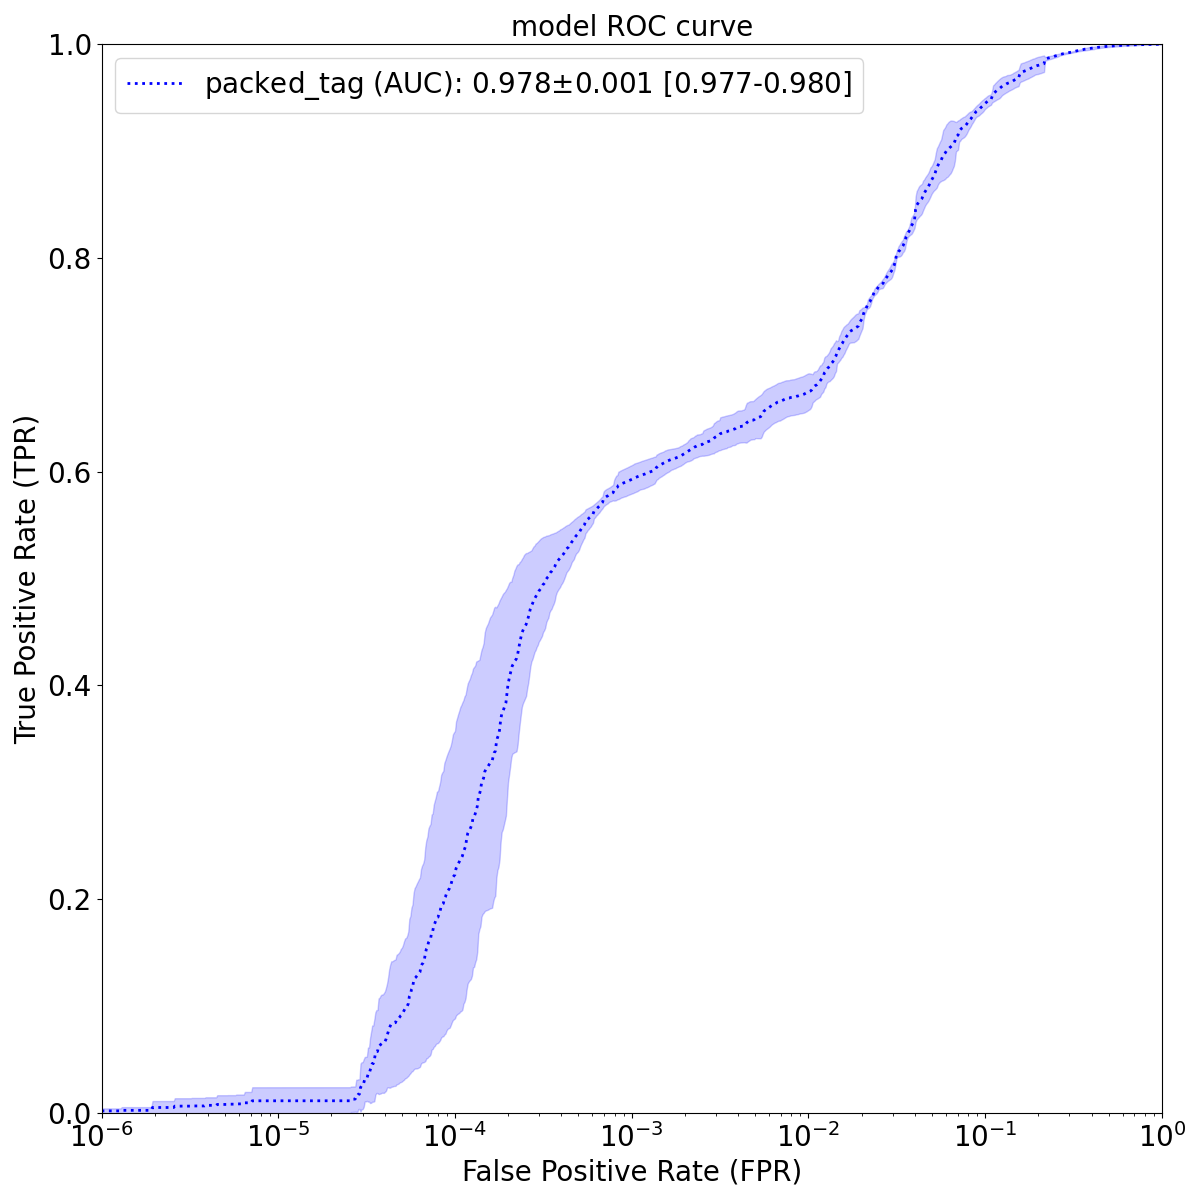
\includegraphics[width=0.6\textwidth]{./results/packed_tag_roc_aloha.png}
        \vspace*{-0.2cm}
        \caption[Packed Tag prediction task ALOHA ROC curve]{ROC curve and AUC statistics of \textBF{ALOHA} model for the \textbf{Packed Tag}. The line represents the \textit{mean} TPR at a given FPR, while the shaded region represents the \textit{standard deviation}. Statistics were computed over \textBF{3} training runs, each with random parameter initialization.}
        \label{fig:packedTagRocAloha}
    \end{figure}
}

\newcommand{\packedTagRocJointEmbedding}{
    \begin{figure}[H]
        \vspace*{-0.5cm}
        \centering
        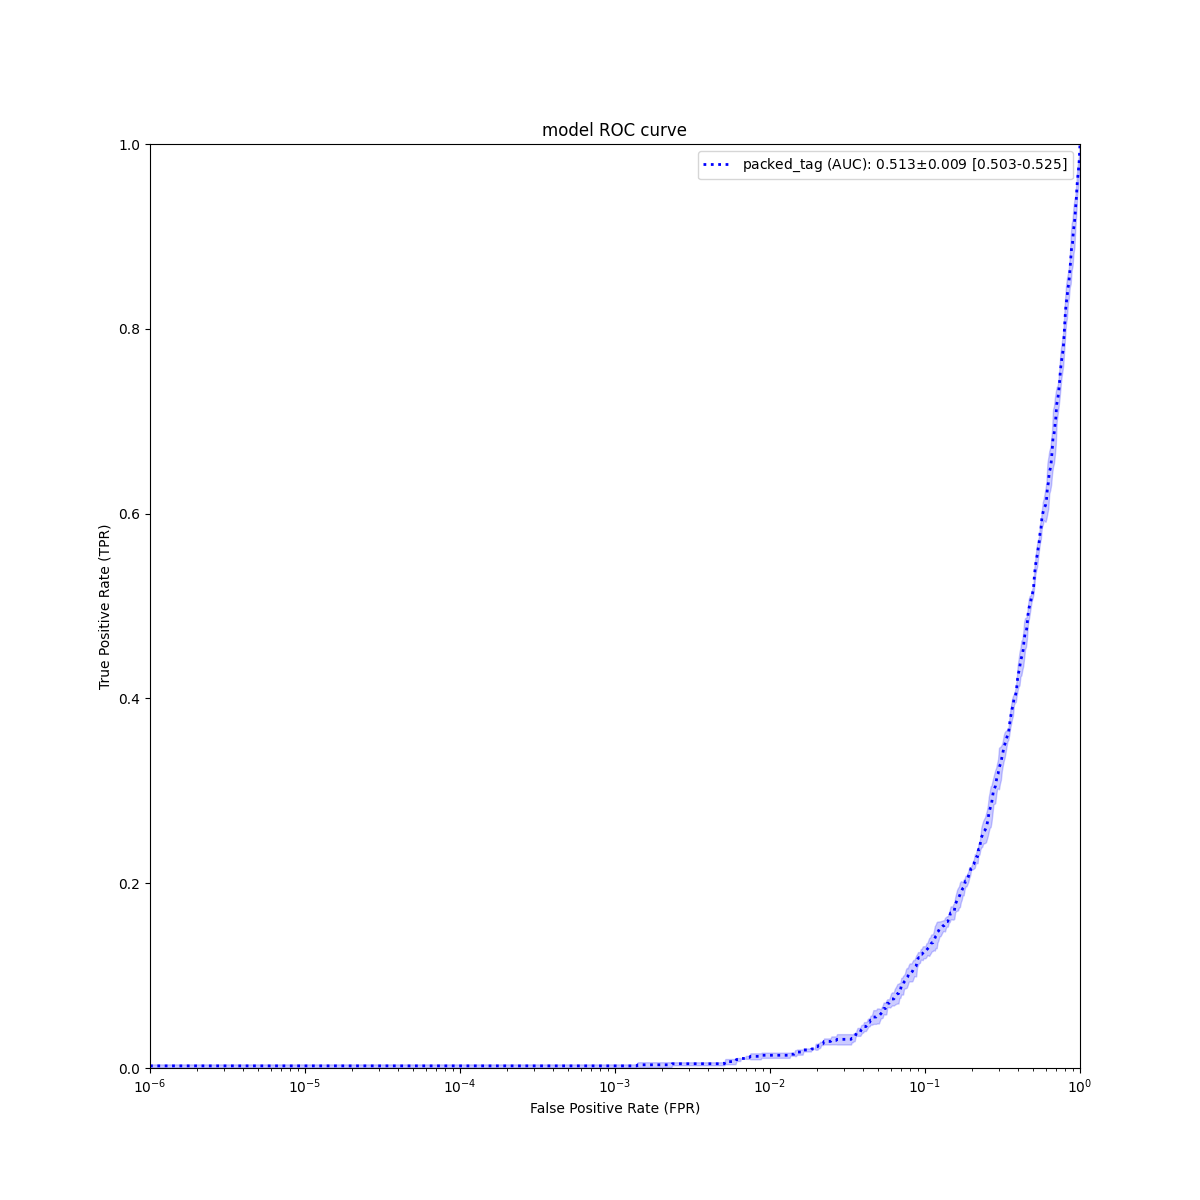
\includegraphics[width=0.6\textwidth]{./results/packed_tag_roc_jointEmbedding.png}
        \vspace*{-0.2cm}
        \caption[Packed Tag prediction task Joint Embedding ROC curve]{ROC curve and AUC statistics of \textBF{Joint Embedding} model for the \textbf{Packed Tag}. The line represents the \textit{mean} TPR at a given FPR, while the shaded region represents the \textit{standard deviation}. Statistics were computed over \textBF{3} training runs, each with random parameter initialization.}
        \label{fig:packedTagRocJointEmbedding}
    \end{figure}
}

\newcommand{\packedTagRocProposedMethod}{
    \begin{figure}[H]
        \vspace*{-0.5cm}
        \centering
        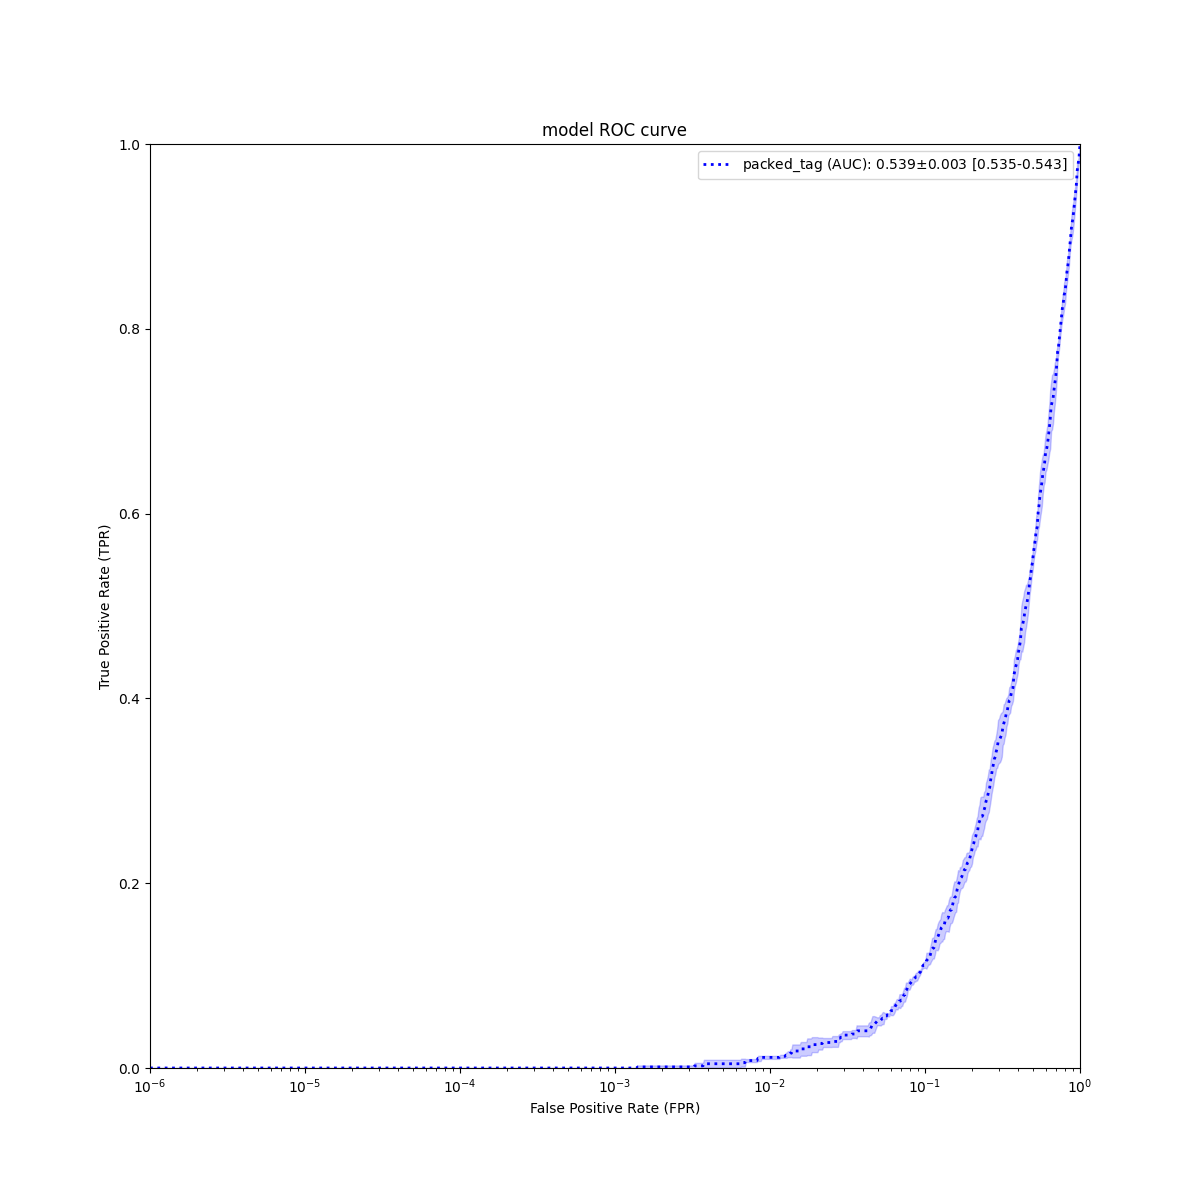
\includegraphics[width=0.6\textwidth]{./results/packed_tag_roc_proposedModel.png}
        \vspace*{-0.2cm}
        \caption[Packed Tag prediction task Proposed Model ROC curve]{ROC curve and AUC statistics of \textBF{Proposed Model} for the \textbf{Packed Tag}. The line represents the \textit{mean} TPR at a given FPR, while the shaded region represents the \textit{standard deviation}. Statistics were computed over \textBF{3} training runs, each with random parameter initialization.}
        \label{fig:packedTagRocProposedModel}
    \end{figure}
}
